\documentclass[12pt,a4paper]{article}
\usepackage{fontspec}
\defaultfontfeatures{Mapping=tex-text}
\usepackage{xunicode}
\usepackage{xltxtra}
\setmainfont{Helvetica}
\newfontfamily{\cyrillicfonttt}{Helvetica}
\newfontfamily{\cyrillicfont}{Helvetica}
\newfontfamily{\cyrillicfontsf}{Helvetica}
\usepackage{polyglossia}
\setdefaultlanguage{russian}
\usepackage{amsmath,amsfonts,amssymb,amsthm,mathtools}       
\usepackage{unicode-math}
\usepackage{leqno}     
\usepackage{graphicx}
\graphicspath{{Pictures/}}
\DeclareGraphicsExtensions{.jpg}
\begin{document}
\section{О себе!}
\begin{enumerate}
\item Меня зовут Даша Францева
\item Учусь на 3 курсе эконома
\item Приехала из Рязани
\item Живу в общаге
\item Занимаюсь танцами
\item Нравится читать детективы
\item Бывает,хожу в театры
\item Люблю путешествия
\item Обожаю Италию и итальянскую еду
\item Хочу успешно освоить LaTex
\end{enumerate}
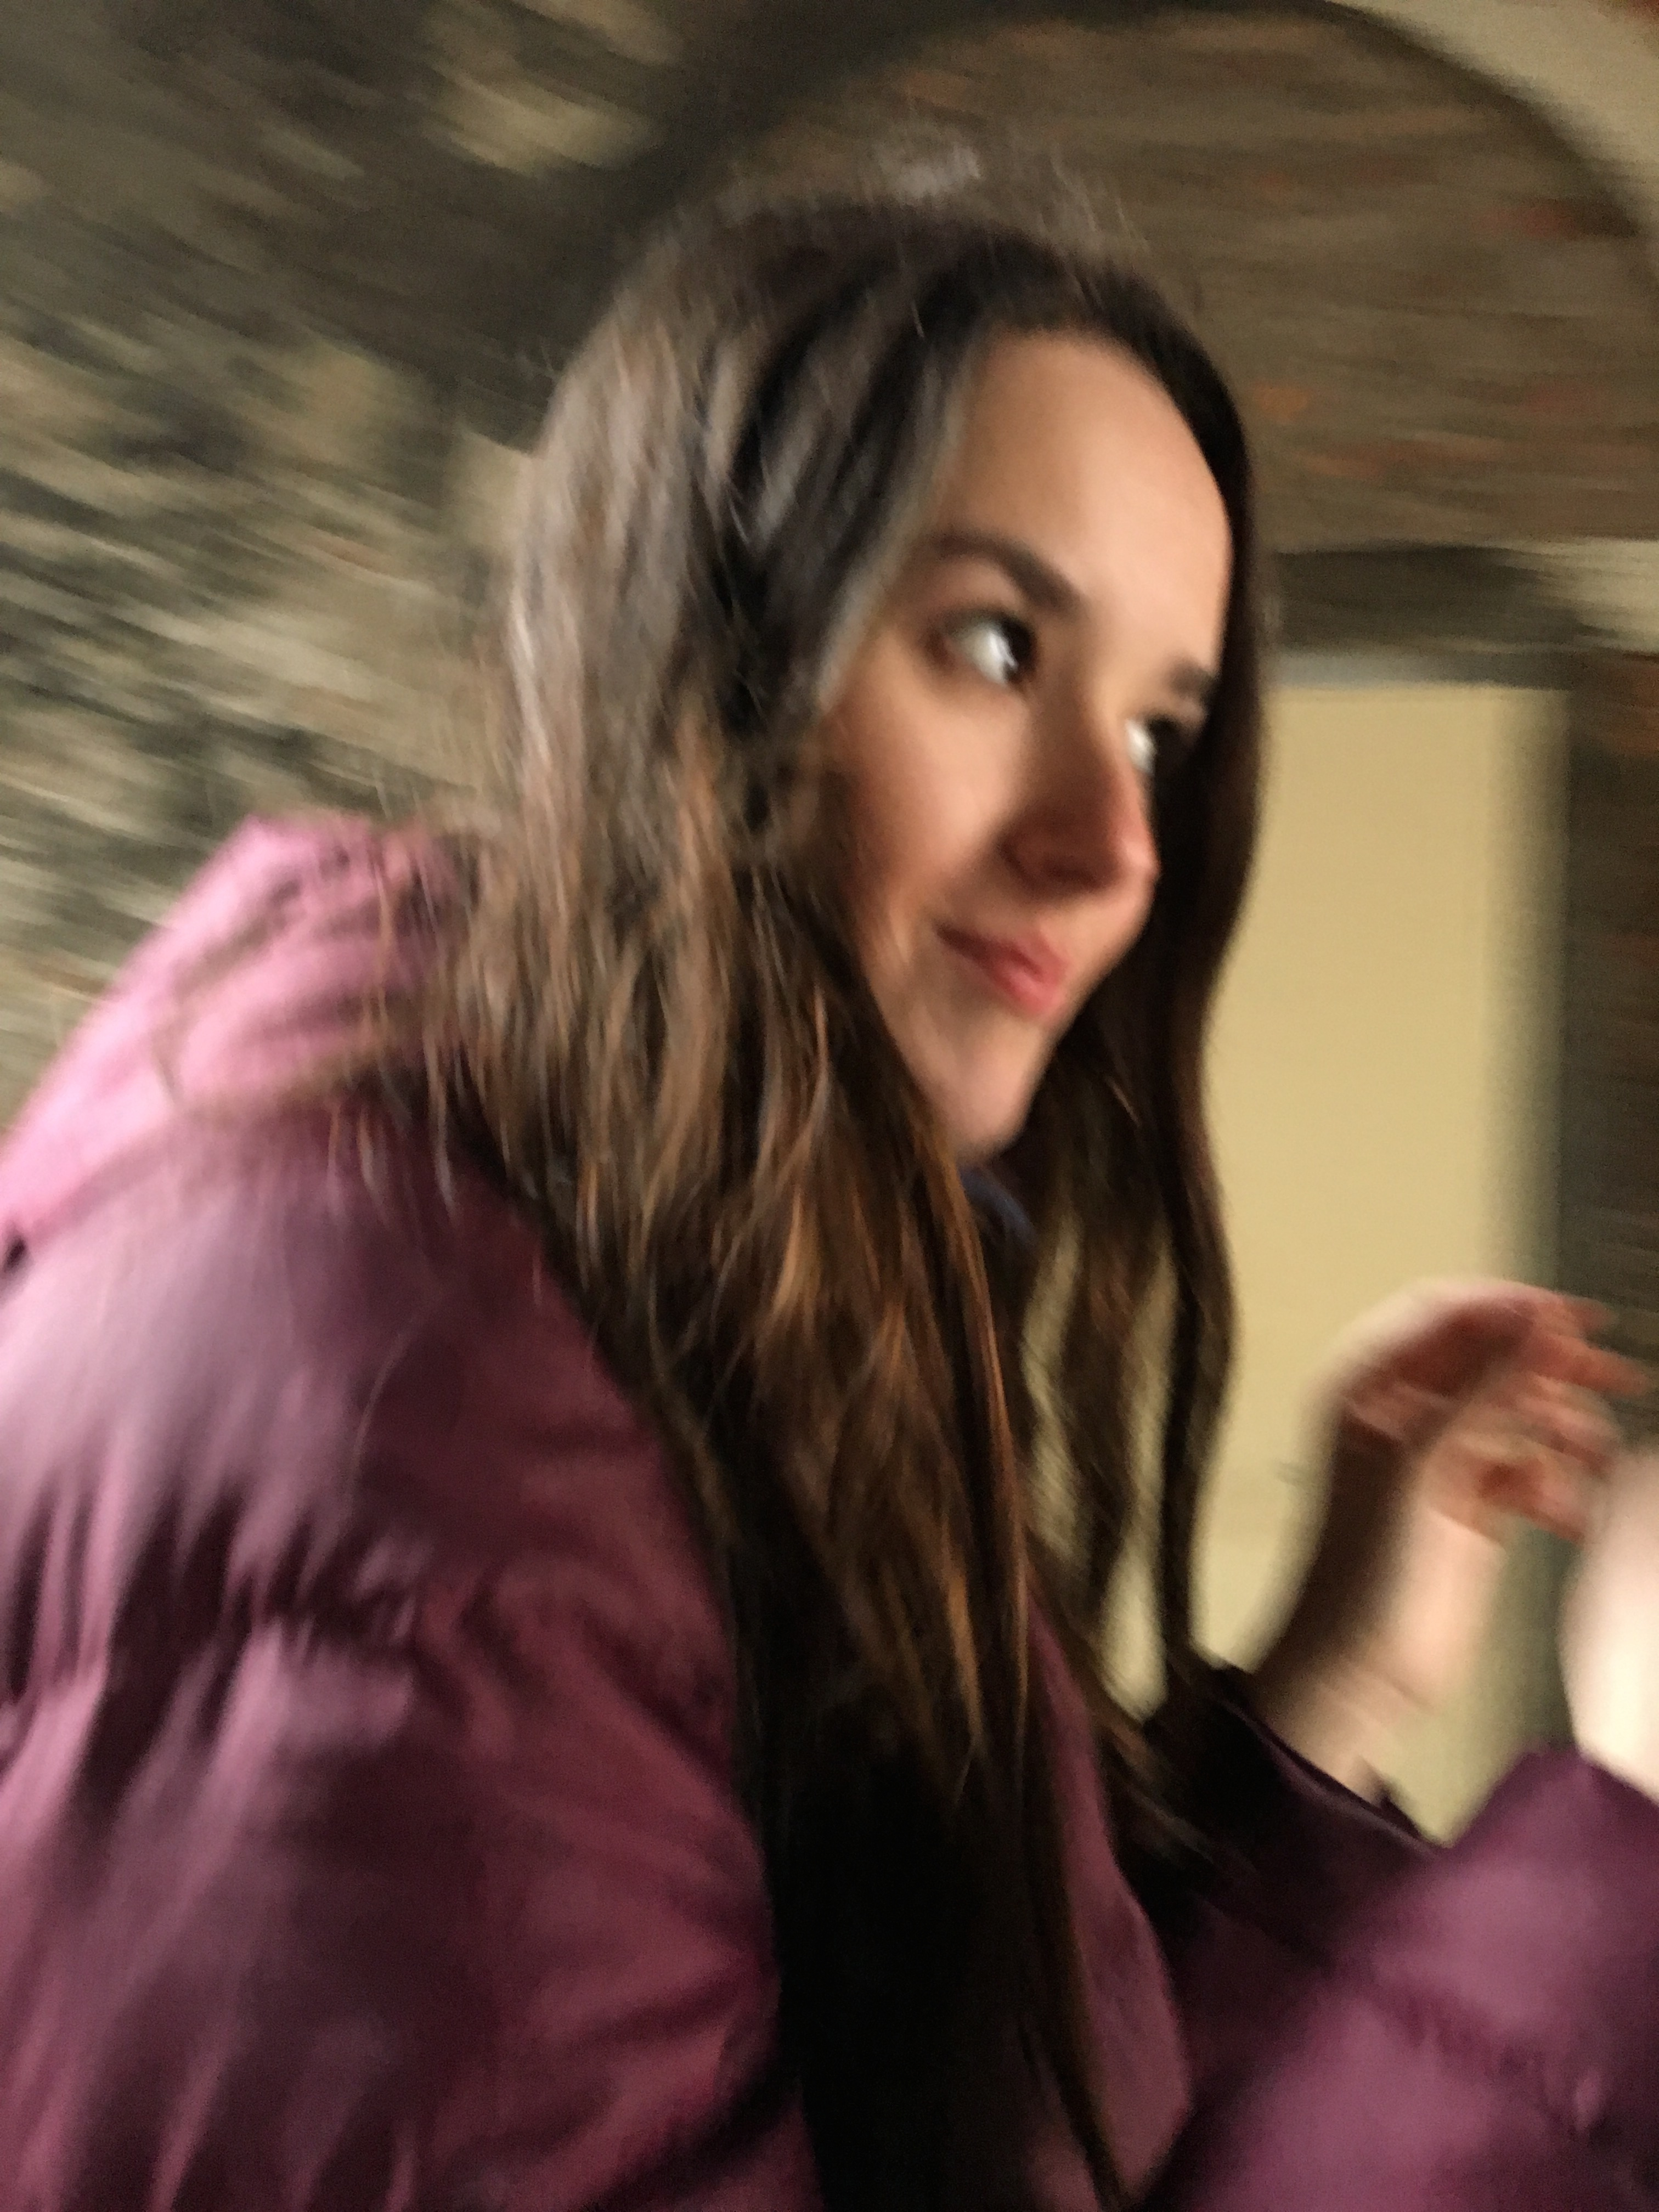
\includegraphics[height=7cm]{IMG_6145}
\section{Формулы}
\subsection{Любимые формулы}
\begin{equation}\label{formula1}
(a+b)^n=a^n + C^1_n \cdot a^{n-1} \cdot b + C^2_n \cdot a^{n-2} \cdot b^2 + \ldots + C^{n-1}_n \cdot a \cdot b^{n-1} + b^n
\end{equation}
\begin{equation}\label{formula2}
	\begin{aligned}
	n(\bigcup_{i=1}^{\infty}A_i) & =\sum_{i=1}^k n(A_i) - [n(A_1 \bigcap A_2) + n(A_1 \bigcap A_3) + \ldots +\\
	& + n(A_{k-1} \bigcap A_k)] +[n(A_1 \bigcap A_2 \bigcap A_3) + n(A_1 \bigcap \\
	& \bigcap A_2 \bigcap A_4) +  \ldots + n(A_{k-2} \bigcap A_{k-1} \bigcap A_k)] - \ldots +\\
	&+(-1)^{k-1} \cdot n(A_1 \bigcap A_2 \bigcap \ldots \bigcap A_n)
	\end{aligned}
\end{equation}
\begin{equation}\label{formula3}
\lim_{x \to 0} \left(\frac{\sin x}{x}\right)=1
\end{equation}
\begin{equation}\label{formula4}
\triangle =
 \begin{vmatrix}
  a_{1,1} & a_{1,2} & \cdots & a_{1,n} \\
  a_{2,1} & a_{2,2} & \cdots & a_{2,n} \\
  \vdots  & \vdots  & \ddots & \vdots  \\
  a_{n,1} & a_{n,2} & \cdots & a_{n,n}
 \end{vmatrix} = \sum_{j=(j_1, \ldots, j_n)}(-1)^{t(j)} \cdot a_{1j_1} \cdot a_{2j_2} \ldots \cdot a_{nj_n}
\end{equation}
\begin{equation}\label{formula5}
\begin{aligned}
f(x)&=f(a)+\frac{f\prime(a)}{1!}\cdot(x-a)+\frac{f\prime\prime(a)}{2!}\cdot(x-a)^2+\ldots+\\
&+\frac{f^{(n)}(a)}{n!}\cdot(x-a)^n+R_n(x)
\end{aligned}
\end{equation}
\subsection{Нелюбимая формула}
\begin{equation}\label{formula6}  
\int\limits_0^\infty
\frac{\sin^2px}{x^2}dx = \frac{\pi \cdot p}{2}
\end{equation}

Бином Ньютона \ref{formula1} мне нравится, так как напоминает о чудесном первом курсе, дискретке и Василии Палыче. Формула \ref{formula2} нравится мне по той же причине. Первый замечательный предел \ref{formula3} невозможно не любить. Формула определителя \ref{formula4} нравится, потому что она легко запоминается и досталась мне на коллоквиуме по линалу. Ряд Тейлора \ref{formula5} не то что бы очень люблю, но часто использовали его и поэтому хорошо к нему отношусь. А вот к интегралам типа \ref{formula6} у меня холодное отношение. И тригонометрию не люблю.

\end{document}